\documentclass[UTF8,fontset=ubuntu]{ctexart}
\usepackage{amsmath}
\usepackage{amssymb}
\usepackage{bm}
\usepackage{cancel}
\usepackage{colortbl}
\usepackage{framed}
\usepackage[framed]{ntheorem}
\usepackage{parskip}
\usepackage{pifont}
\usepackage{tikz}
\usepackage{xcolor}
\theoremheaderfont{\normalfont\bfseries}
\theorembodyfont{\slshape}
\theoremseparator{\hspace{2ex}}
\theoremindent2ex
\theoremstyle{plain}
\newtheorem{theorem}{定理}
\theoremstyle{nonumberplain}
\newtheorem{definition}{定义}
\theoremstyle{empty}
\newframedtheorem{law}{定律}
\definecolor{lightgray}{gray}{0.7}
\definecolor{gray}{gray}{0.5}
\definecolor{white}{gray}{1}
\renewcommand{\thesection}{}
\begin{document}
\part{线性代数中的线性方程组}
\section{一、线性方程组}
线性方程:
	\[ a_{1}x_{1}+a_{2}x_{2}+\cdots +a_{n}x_{n}=b \]
其中, $b$与系数$a_{1}$,$a_{2}$,$\cdots$,$a_{n}$是实数或复数, 通常为已知数. n为任意正整数\\[2ex]

线性方程组 -- 由一个或几个包含相同变量的线性方程组成, 如:
\[\left\{\begin{array}{r@{\hspace{1.5pt}}l@{\hspace{1.5pt}}r@{\hspace{1.5pt}}l@{\hspace{1.5pt}}r@{\hspace{1.5pt}}l@{\hspace{1.5pt}}r}
	2x_1 & - & x_2 & + & 1.5x_3 & = & 8\\
	x_1  &   &     & - & 4x_3   & = & -7		
\end{array}\right.\]
若线性方程组的方程个数少于未知数个数, 称之为\textbf{欠定方程组}\\
若线性方程组的方程个数多余未知数个数, 称之为\textbf{超定方程组}\\
方程组所有可能的解的集合称为线性方程组的\textbf{解集}\\
若两个方程组有相同的解集, 则这两个方程组称为\textbf{等价}的\\[2ex]

线性方程组解集情况:\\
1.无解;\\
2.有唯一解;\\
3.有无穷多解.\\[1ex]
当方程组无解时, 称线性方程组\textbf{不相容}\\
当方程组有唯一解或无穷多解时, 称线性方程组\textbf{相容}\\[2ex]

线性方程组
\[\left\{\begin{array}{r@{\hspace{1.5pt}}l@{\hspace{1.5pt}}r@{\hspace{1.5pt}}l@{\hspace{1.5pt}}r@{\hspace{1.5pt}}l@{\hspace{1.5pt}}r}
x_1 & - & 2x_2 & + &  x_3 & = & 0\\
	& 	& 2x_2 & - & 8x_3 & = & 8\\
-4x_1 & + & 5x_2 & + & 9x_3 & = & -9
\end{array}\right.\]
线性方程组的\textbf{系数矩阵}
\[\left[\begin{array}{r r r}
	1 & -2 & 1\\
	0 & 2  & -8\\
	-4 & 5 & 9
\end{array}\right]\]
线性方程组的\textbf{增广矩阵}
\[\left[\begin{array}{r r r r}
	1 & -2 & 1 & 0\\
	0 & 2  & -8 & 8\\
	-4 & 5 & 9 & -9
\end{array}\right]\]\\[2ex]

解线性方程组\\
思路: 将方程组用一个更容易求解的等价方程组替代\\

化简方程组的三种基本变换:\\
1.倍加变换 - 将某方程替换为它与另一方程倍数的和;\\
2.对换变换 - 交换两个方程的位置;\\
3.倍乘变换 - 方程的所有系数乘以一个非0实数.\\

例. 简化如下方程组
\[\begin{array}{r@{\hspace{1.5pt}}l@{\hspace{1.5pt}}r@{\hspace{1.5pt}}l@{\hspace{1.5pt}}r@{\hspace{1.5pt}}l@{\hspace{1.5pt}}r}
x_1 & - & 2x_2 & + &  x_3 & = & 0\\
	& 	& 2x_2 & - & 8x_3 & = & 8\\
-4x_1 & + & 5x_2 & + & 9x_3 & = & -9
\end{array}\qquad\left[\begin{array}{r r r r}
	1 & -2 & 1 & 0\\
	0 & 2 & -8 & 8\\
	-4 & 5 & 9 & -9
\end{array}\right]\]
步骤1 -- \ding{194}+4\ding{192}
\[\left[\begin{array}{r r r r}
    1 & -2 & 1 & 0\\
    0 & 2 & -8 & 8\\
    -4 & 5 & 9 & -9
\end{array}\right] \Rightarrow \left[\begin{array}{r r r r}
    1 & -2 & 1 & 0\\
    0 & 2 & -8 & 8\\
    0 & -3 & 13 & -9
\end{array}\right]\]
步骤2 -- $\dfrac{1}{2}$\ding{193}
\[\left[\begin{array}{r r r r}
    1 & -2 & 1 & 0\\
    0 & 2 & -8 & 8\\
    0 & -3 & 13 & -9
\end{array}\right] \Rightarrow \left[\begin{array}{r r r r}
    1 & -2 & 1 & 0\\
    0 & 1 & -4 & 4\\
    0 & -3 & 13 & -9
\end{array}\right]\]
步骤3 -- \ding{194}+3\ding{193}
\[\left[\begin{array}{r r r r}
    1 & -2 & 1 & 0\\
    0 & 1 & -4 & 4\\
    0 & -3 & 13 & -9
\end{array}\right] \Longrightarrow \left[\begin{array}{r r r r}
	1 & -2 & 1 & 0\\
	0 & 1 & -4 & 4\\
	0 & 0 & 1 & 3
\end{array}\right]\]
步骤4 -- \ding{193}+4\ding{194}
\[\left[\begin{array}{r r r r}
    1 & -2 & 1 & 0\\
    0 & 1 & -4 & 4\\
    0 & 0 & 1 & 3
\end{array}\right] \Longrightarrow \left[\begin{array}{r r r r}
	1 & -2 & 1 & 0\\
	0 & 1 & 0 & 16\\
	0 & 0 & 1 & 3
\end{array}\right]\]
步骤5 -- \ding{192}+(-\ding{194})
\[\left[\begin{array}{r r r r}
    1 & -2 & 1 & 0\\
    0 & 1 & 0 & 16\\
    0 & 0 & 1 & 3
\end{array}\right] \Longrightarrow \left[\begin{array}{r r r r}
	1 & -2 & 0 & -3\\
	0 & 1 & 0 & 16\\
	0 & 0 & 1 & 3
\end{array}\right]\]
步骤6 -- \ding{192}+2\ding{193}
\[\left[\begin{array}{r r r r}
    1 & -2 & 0 & -3\\
    0 & 1 & 0 & 16\\
    0 & 0 & 1 & 3
\end{array}\right] \Longrightarrow \left[\begin{array}{r r r r}
	1 & 0 & 0 & 29\\
	0 & 1 & 0 & 16\\
	0 & 0 & 1 & 3
\end{array}\right]\]
\framebox{若两个线性方程组的增广矩阵是行等价的, 则它们具有相同的解集}\vspace{6ex}

\section{二、行化简与阶梯形矩阵}
非零行(列): 矩阵中至少包含一个非零元素的行(列)\\
先导元素: 该行最左边的非零元素\\
\begin{definition}
一个矩阵称为阶梯形, 若它有以下三个性质:\\
1.所有非零行在零行之上;\\
2.某一行先导元素的列位于上一行先导元素的右边;\\
3.某一先导元素所在列下方元素都是零;\\
若还满足以下性质, 则称为简化阶梯形:\\
4.每一非零行的先导元素是1;\\
5.每一先导元素是该元素所在列的唯一非零元素.
\end{definition}\vspace{2ex}

\begin{theorem}[简化阶梯形矩阵的唯一性]
每个矩阵行等价于唯一的简化阶梯形矩阵.
\end{theorem}\vspace{2ex}

\begin{definition}
矩阵A中的{\heiti 主元位置}是A中对应于它的阶梯形中先导元素的位置.{\heiti 主元列}是A中含有主元位置的列.
\end{definition}\vspace{2ex}

基本变量: 位于主元列的变量\\
自由变量: 位于非主元列的变量\\[2ex]

\begin{theorem}[存在与唯一性定理]
线性方程组相容的充要条件是增广矩阵的最右列不是主元列. 也就是说, 增广矩阵的阶梯形没有形如
	\[[0\ \cdots\ 0\ b], b\neq 0\]
的行. 若线性方程组相容, 则它的解集可能有两种情形:\\
1)当没有自由变量时, 有唯一解;\\
2)若至少有一个自由变量, 则有无穷多解.
\end{theorem}\vspace{2ex}

应用行化简算法解线性方程组:\\
1.写出方程组的增广矩阵\\
2.应用行化简算法把增广矩阵化为阶梯形, 确定方程组是否相容, 如果没有解则停止; 否则进行下一步\\
3.继续行化简算法得到它的简化阶梯形\\
4.写出简化阶梯形矩阵对应的方程组\\
5.将每个非零方程改写为使用自由变量表示基本变量的形式\\[4ex]

\section{三、向量方程}
列向量: 仅含一列的矩阵, 简称为向量. 如:
\[u=\left[\begin{array}{c}
	3\\
	-1
\end{array}\right] \text{\quad or\quad} u=(3, -1)\]\\[2ex]
行向量: 仅含一行的矩阵. 如:
\[v=\left[\begin{array}{c c}
	2 & 5
\end{array}\right]\]\\[2ex]
所有两个元素的向量表示为$\mathbb{R}^2$, $\mathbb{R}$表示元素为实数, 2表示向量包含两个元素\\
向量加法:
\begin{equation*}
\left[\begin{array}{c}
	1\\
	-2
\end{array}\right]
+
\left[\begin{array}{c}
	2\\
	5
\end{array}\right]
=
\left[\begin{array}{c}
	1+2\\
	-2+5
\end{array}\right]
=
\left[\begin{array}{c}
	3\\
	3
\end{array}\right]
\end{equation*}
标量乘法:\\
\indent 若$u=\left[\begin{array}{c}3\\-1\end{array}\right]$, $c=5$, 则:
\[cu=5\left[\begin{array}{c}3\\-1\end{array}\right]=\left[\begin{array}{c}15\\-5\end{array}\right]\]

向量$\left[\begin{array}{r}x\\y\end{array}\right]$的几何含义: 由原点(0,0)指向点(x,y)的有向线段\\[2ex]

\begin{law}[向量加法的平行四边形法则]\ \\
若$\mathbb{R}^2$中向量$\mathbf{u}$和$\mathbf{v}$用平面上的点表示, 则$\mathbf{u+v}$对应于以$\mathbf{u}$,$\mathbf{0}$和$\mathbf{v}$为三个顶点的平行四边形的第4个顶点, 如图.\\[2ex]
\begin{center}
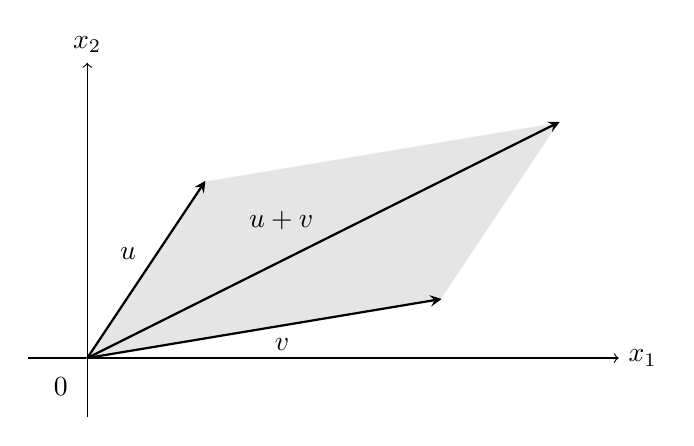
\begin{tikzpicture}[scale=0.75]
\draw[->] (-1,0) -- (9,0) node[right]{$x_1$};
\draw[->] (0,-1) -- (0,5) node[above]{$x_2$};
\draw[color=white, fill=black!10] (0,0) -- (6,1) -- (8,4) -- (2,3) -- cycle;
\draw[-stealth, thick, auto] (0,0) -- (2,3) node[pos=0.5]{$u$};
\draw[-stealth, thick, auto, swap] (0,0) -- (6,1) node[pos=0.5]{$v$};
\draw[-stealth, thick, auto] (0,0) -- (8,4) node[pos=0.5]{$u+v$};
\node at (0,0) [label=below left:$0$]{};
\end{tikzpicture}
\end{center}
\end{law}\vspace{3ex}

所有元素都是零的向量称为\textbf{零向量}, 用\textbf{0}表示(\textbf{0}中元素的个数可由上下文确定)\\[2ex]

\begin{law}[$\mathbb{R}^n$中向量的代数性质]\ \\
对$\mathbb{R}^n$中一切向量$\mathbf{u}$,$\mathbf{v}$,$\mathbf{w}$以及标量$c$和$d$:
\begin{equation*}
\begin{array}{l@{}c@{}l l l@{}c@{}l l}
( & i & ) & \mathbf{u}+\mathbf{v}=\mathbf{v}+\mathbf{u} & ( & v & ) & c(\mathbf{u}+\mathbf{v})=c\mathbf{u}+c\mathbf{v}\\
( & ii & ) & (\mathbf{u}+\mathbf{v})+\mathbf{w}=\mathbf{u}+(\mathbf{v}+\mathbf{w}) & ( & vi & ) & (c+d)\mathbf{u}=c\mathbf{u}+d\mathbf{u}\\
( & iii & ) & \mathbf{u}+\mathbf{0}=\mathbf{0}+\mathbf{u}=\mathbf{u} & ( & vii & ) & c(d\mathbf{u})=(cd)\mathbf{u}\\
( & iv & ) & \mathbf{u}+(-\mathbf{u})=-\mathbf{u}+\mathbf{u}=\mathbf{0} & ( & viii & ) & 1\mathbf{u}=\mathbf{u}
\end{array}
\end{equation*}
\end{law}\vspace{2ex}

给定$\mathbb{R}^n$中向量$\mathbf{v}_1$,$\mathbf{v}_2$,$\cdots$,$\mathbf{v}_p$和标量$c_1$,$c_2$,$\cdots$,$c_p$, 向量
	\[\mathbf{y}=c_1\mathbf{v}_1+\cdots+c_p\mathbf{v}_p\]
称为向量$\mathbf{v}_1$,$\mathbf{v}_2$,$\cdots$,$\mathbf{v}_p$以$c_1$,$c_2$,$\cdots$,$c_p$为\textbf{权}的\textbf{线性组合}.\\[2ex]

\framebox{
\begin{minipage}{\linewidth}
向量方程
\[x_1\mathbf{a}_1+x_2\mathbf{a}_a+\cdots+x_n\mathbf{a}_n=\mathbf{b}\]
和增广矩阵为
\begin{equation}
[\mathbf{a}_1\quad\mathbf{a}_2\quad\cdots\quad\mathbf{a}_n\quad\mathbf{b}]\label{matrix:eq_01}
\end{equation}
的线性方程组有相同的解集. 特别地, $\mathbf{b}$可表示为$\mathbf{a}_1$,$\mathbf{a}_2$,$\cdots$,$\mathbf{a}_n$的线性组合当且仅当对应于\eqref{matrix:eq_01}式的线性方程组有解.
\end{minipage}}\\[4ex]

\begin{definition}
若$\mathbf{v}_1$,$\mathbf{v}_2$,$\cdots$,$\mathbf{v}_p$是$\mathbb{R}^n$中的向量, 则$\mathbf{v}_1$,$\mathbf{v}_2$,$\cdots$,$\mathbf{v}_p$的所有线性组合所成的组合用记号Span\{$\mathbf{v}_1$,$\mathbf{v}_2$,$\cdots$,$\mathbf{v}_p$\}表示, 称为\textbf{$\text{由}\mathbf{v}_1,\mathbf{v}_2,\cdots,\mathbf{v}_p\text{所生成的(\textmd{或}张成)}\mathbb{R}^n\text{的子集}$}. 也就是说, Span\{$\mathbf{v}_1$,$\mathbf{v}_2$,$\cdots$,$\mathbf{v}_p$\}是所有形如
	\[c_1\mathbf{v}_1+c_2\mathbf{v}_2+\cdots+c_p\mathbf{v}_p\]
的向量的集合, 其中$c_1$,$c_2$,$\cdots$,$c_p$为标量.\\[2ex]
\end{definition}\vspace{4ex}

\section{四、矩阵方程$A\mathbf{x}=\mathbf{b}$}
\begin{definition}
若$A$是$m\times n$矩阵, 它的各列为$\bm{a}_1$,$\cdots$,$\bm{a}_n$. 若$\bm{x}$是$\mathbb{R}^n$中的向量, 则\textbf{$A$与$\bm{x}$的积}(记为$A\bm{x}$)就是\textbf{$A$的各列以$\bm{x}$中对应元素为权的线性组合}, 即
	\[A\bm{x}=[\bm{a}_1\ \bm{a}_2\ \cdots\ \bm{a}_n]\left[\begin{array}{c}x_1\\x_2\\\vdots\\x_n\end{array}\right]=x_1\bm{a}_1+x_2\bm{a}_2+\cdots+x_n\bm{a}_n\]
注意$A\bm{x}$仅当$A$的列数等于$\bm{x}$中的元素个数时才有意义.\\[2ex]
\end{definition}

\begin{theorem}
若$A$是$m\times n$矩阵, 它的各列为$\bm{a}_1$,$\cdots$,$\bm{a}_n$, 而$\bm{b}$属于$\mathbb{R}^n$, 则矩阵方程
\[A\bm{x}=\bm{b}\]
与向量方程
\[x_1\bm{a}_1+x_2\bm{a}_2+\cdots+x_n\bm{a}_n=\bm{b}\]
有相同的解集. 它又与增广矩阵为
\[[\bm{a}_1\ \bm{a}_2\ \cdots\ \bm{a}_n\ \bm{b}]\]
的线性方程组有相同的解集.\\[2ex]
\end{theorem}\vspace{2ex}

\begin{theorem}
设$A$是$m\times n$矩阵, 则下列命题是逻辑上等价的. 也就是说, 对某个$A$, 它们都成立或者都不成立.\\
\begin{tabular}{l@{\,}l}
a. & 对$\mathbb{R}^m$中每个$\bm{b}$, 方程$A\bm{x}=\bm{b}$有解.\\
b. & $\mathbb{R}^m$中的每个$\bm{b}$都是$A$的列的一个线性组合.\\
c. & $A$的各列生成$\mathbb{R}^m$.\\
d. & $A$在每一行都有一个主元位置.\\[2ex]
\end{tabular}
\end{theorem}\vspace{2ex}

\begin{law}[计算$A\bm{x}$的行--向量规则]\ \\
若乘积$A\bm{x}$有定义, 则$A\bm{x}$中的第$i$个元素是$A$的第$i$行元素与$\bm{x}$的相应元素乘积之和.
\end{law}\vspace{2ex}

矩阵的主对角线上元素为1, 其他位置上元素为0, 这个矩阵称为\textbf{单位矩阵}, 并记为$I$.\\
如果矩阵为$n\times n$单位矩阵, 记为$I_n$.\\[2ex]

\begin{theorem}
若$A$是$m\times n$矩阵, $\bm{u}$和$\bm{v}$是$\mathbb{R}^n$中向量, c是标量, 则\\
\begin{tabular}{l@{\,}l}
a. & $A(\bm{u}+\bm{v})=A\bm{u}+A\bm{v}$\\
b. & $A(c\bm{u})=c(A\bm{u})$
\end{tabular}
\end{theorem}\vspace{6ex}

\section{五、线性方程组的解集}
若线性方程组可写成
\[A\bm{x}=\bm{0}\]
的形式, 则称为\textbf{齐次线性方程组}. 其中, $A$是$m\times n$矩阵, $\bm{0}$是$\mathbb{R}^m$中的零向量.\\
齐次线性方程组至少有一个解, 即$\bm{x}=\bm{0}$($\mathbb{R}^n$中的零向量), 这个解称为它的\textbf{平凡解}.\\
如果有一个非零向量$\bm{x}$, 满足$A\bm{x}=\bm{0}$, 这个解称为它的\textbf{非平凡解}.\\[2ex]

\begin{law}
齐次方程$A\bm{x}=\bm{0}$有非平凡解当且仅当方程至少有一个自由变量.
\end{law}\vspace{2ex}

$\bm{x}=s\bm{u}+t\bm{v}$为$A\bm{x}=\bm{0}$的\textbf{参数向量形式}, 并称之为\textbf{参数向量方程}. 其中, $s$,$t$为自由变量\\
$\bm{x}=\bm{p}+t\bm{v}$为$A\bm{x}=\bm{b}$的\textbf{参数向量形式}, 并称之为\textbf{参数向量方程}. 其中, $t$为自由变量\\
例.\\
$x_1=0.3x_2+0.2x_3$\\[1ex]
$\bm{x}=
\left[\begin{array}{l}
x_1\\
x_2\\
x_3
\end{array}\right]=
\left[\begin{array}{c}
0.3x_2+0.2x_3\\
x_2\\
x_3
\end{array}\right]=
\left[\begin{array}{r}
0.3x_2\\
x_2\\
0
\end{array}\right]+\left[\begin{array}{r}
0.2x_3\\
0\\
x_3
\end{array}\right]\\
\phantom{\bm{x}}=x_2\left[\begin{array}{r}
0.3\\
1\\
0
\end{array}\right]+x_3\left[\begin{array}{r}
0.2\\
0\\
1
\end{array}\right]
$\\[1ex]
因此, $A\bm{x}=\bm{b}$的解集是一条通过$\bm{p}$而平行于$A\bm{x}=\bm{0}$的解集的直线. 也称为将$\bm{v}$沿着$\bm{p}$进行直线移动.\\[2ex]

\begin{theorem}
设方程$A\bm{x}=\bm{b}$对某个$\bm{b}$是相容的, $\bm{p}$为一个特解, 则$A\bm{x}=\bm{b}$的解集是所有形如$\bm{w}=\bm{p}+\bm{v}_h$的向量的集, 其中$\bm{v}_h$时齐次方程$A\bm{x}=\bm{b}$的任意一个解.
\end{theorem}\vspace{3ex}

\begin{law}[把(相容方程组的)解集表示成参数向量形式]\ \\
1.把增广矩阵简化为简化阶梯形.\\
2.把每个基本变量用自由变量表示.\\
3.把一般解$\bm{x}$表示成向量, 如果有自由变量, 其元素依赖于自由变量.\\
4.把$\bm{x}$分解为向量(元素为常数)的线性组合, 用自由变量作为参数.
\end{law}\vspace{4ex}

\section{六、线性方程组的应用}
1.经济学 - 部分的收支平衡\\
2.化学式 - 等号两边原子守恒\\
3.网络流 - 节点的进/出流量恒等\\[4ex]

\section{七、线性无关}
\begin{definition}
$\mathbb{R}^n$中一组向量\{$\bm{v}_1$,$\cdots$,$\bm{v}_p$\}称为\textbf{线性无关}的, 若向量方程
\[x_1\bm{v}_1+x_2\bm{v}_2+\cdots+x_p\bm{v}_p=\bm{0}\]
仅有平凡解. 向量组(集)\{$\bm{v}_1$,$\cdots$,$\bm{v}_p$\}称为\textbf{线性相关}的, 若存在不全为零的权$c_1$,$\cdots$,$c_p$, 使
\[c_1\bm{v}_1+c_2\bm{v}_2+\cdots+c_p\bm{v}_p=\bm{0}\]
\end{definition}\vspace{2ex}

\begin{law}
矩阵$A$的各列线性无关, 当且仅当方程$A\bm{x}=\bm{0}$仅有平凡解.
\end{law}\vspace{2ex}

\begin{law}
两个向量的集合\{$\bm{v}_1$,$\bm{v}_2$\}线性相关, 当且仅当其中一个向量是另一个向量的倍数. 这个集合线性无关, 当且仅当其中任一个向量都不是另一个向量的倍数.
\end{law}\vspace{4ex}

\begin{theorem}[线性相关集的特征]
两个或更多个向量的集合$S=\{\bm{v}_1,\cdots,\bm{v}_p\}$线性相关, 当且仅当S中至少有一个向量是其他向量的线性组合. 事实上, 若S线性相关, 且$\bm{v}_1\neq\bm{0}$, 则某个$\bm{v}_j$($j>1$)是它前面向量$\bm{v}_1$,$\cdots$,$\bm{v}_{j-1}$的线性组合.
\end{theorem}\vspace{4ex}

\begin{theorem}
若一个向量组的向量个数超过每个向量的元素个数, 那么这个向量组线性相关. 就是说, $\mathbb{R}^n$中任意向量组\{$\bm{v}_1$,$\cdots$,$\bm{v}_p$\}当$p>n$时线性相关.
\end{theorem}\vspace{4ex}

\begin{theorem}
若$\mathbb{R}^n$中向量组$S=\{\bm{v}_1,\cdots,\bm{v}_p\}$包含零向量, 则它线性相关.
\end{theorem}\vspace{4ex}

\section{八、线性变换介绍}
由$\bm{x}$到$A\bm{x}$的对应是由一个向量集到另一个向量集的函数\\[2ex]

\begin{definition}
变换(或映射)$T$称为\textbf{线性}的, 若\\
\begin{tabular}{l@{}c@{}l@{}l}
( & i & ) & 对$T$的定义域中一切$\bm{u}$,$\bm{v}$,$T(\bm{u}+\bm{v})=T(\bm{u})+T(\bm{v})$.\\
( & ii & ) & 对$T$的定义域中的一切$\bm{u}$和数$c$, $T(c\bm{u})=cT(\bm{u})$.
\end{tabular}
\end{definition}\vspace{4ex}

\begin{law}
若T是线性变换, 则
\[T(\bm{0})=\bm{0}\]
且对$T$的定义域中一切向量$\bm{u}$和$\bm{v}$以及数$c$和$d$, 有:
\[T(c\bm{u}+d\bm{v})=cT(\bm{u})+dT(\bm{v})\]
\end{law}\vspace{6ex}

\section{九、线性变换的矩阵}
\begin{theorem}
设$T$:$\mathbb{R}^n\rightarrow\mathbb{R}^m$为线性变换, 则存在唯一的矩阵$A$, 使得对$\mathbb{R}^n$中一切$\bm{x}$, 有
\[T(\bm{x})=A\bm{x}\]
事实上, $A$是$m\times n$矩阵, 它的第$j$列是向量$T(\bm{e}_j)$, 其中$\bm{e}_j$是$\mathbb{R}^n$中单位矩阵$\bm{I}_n$的第$j$列:
\[A=[T(\bm{e}_1)\ \cdots\ T(\bm{e}_n)]\]
\end{theorem}\vspace{4ex}

\begin{definition}
映射$T$:$\mathbb{R}^n\rightarrow\mathbb{R}^m$称为到$\mathbb{R}^m$上的映射, 若$\mathbb{R}^m$中每个$\bm{b}$是$\mathbb{R}^n$中至少一个$\bm{x}$的像.(也称为\textbf{满射}.)
\end{definition}\vspace{4ex}

\begin{definition}
映射$T$:$\mathbb{R}^n\rightarrow\mathbb{R}^m$称为\textbf{一对一映射}(或1:1), 若$\mathbb{R}^m$中每个$\bm{b}$是$\mathbb{R}^n$中至多一个$\bm{x}$的像.(也称为\text{单射}.)
\end{definition}\vspace{4ex}

\begin{theorem}
设$T$:$\mathbb{R}^n\rightarrow\mathbb{R}^m$为线性变换, 则$T$是一对一的当且仅当方程$A\bm{x}=\bm{0}$仅有平凡解.
\end{theorem}\vspace{4ex}

\begin{theorem}
设$T$:$\mathbb{R}^n\rightarrow\mathbb{R}^m$是线性变换, 设$A$为$T$的标准矩阵, 则\\
\begin{tabular}{l@{\ }l}
a. & $T$把$\mathbb{R}^n$映上到$\mathbb{R}^m$, 当且仅当$A$的列生成$\mathbb{R}^m$.\\
b. & $T$是一对一的, 当且仅当$A$的列线性无关.
\end{tabular}
\end{theorem}\vspace{6ex}

\section{十、商业、科学和工程中的线性模型}
\begin{law}[基尔霍夫电压定律]\ \\
围绕一条回路同一方向的电压降$RI$的代数和等于围绕该回路的同一方向电动势的代数和.
\end{law}\vspace{4ex}

\begin{law}
如果有矩阵$A$使$\bm{x}_1=A\bm{x}_0$,$\bm{x}_2=A\bm{x}_1$, 一般地,
\[\bm{x}_{k+1}=A\bm{x}_k\text{,\ }k=0,1,2,\cdots\]
则称为\textbf{线性差分方程}(或\textbf{递归关系}).
\end{law}
\documentclass[UTF8,fontset=ubuntu]{ctexart}
\usepackage{amsmath}
\usepackage{bm}
\usepackage{parskip}
\usepackage{amssymb}
\usepackage{xcolor}
\usepackage{colortbl}
\usepackage{framed}
\usepackage[framed]{ntheorem}
\theoremheaderfont{\normalfont\bfseries}
\theorembodyfont{\slshape}
\theoremseparator{\hspace{2ex}}
\theoremindent2ex
\theoremstyle{plain}
\newtheorem{theorem}{定理}
\theoremstyle{nonumberplain}
\newtheorem{definition}{定义}
\theoremstyle{empty}
\newframedtheorem{law}{定律}
\definecolor{lightgray}{gray}{0.7}
\definecolor{gray}{gray}{0.5}
\definecolor{white}{gray}{1}
\begin{document}
一、矩阵运算\\[1ex]
$m\times n$矩阵$A=[a_{ij}]$的\textbf{对角线元素}是$a_{11}$,$a_{22}$,$a_{33}$,$\cdots$, 它们组成$A$的\textbf{主对角线}.\\[1ex]
\textbf{对角矩阵}是一个方阵, 它的非对角线元素全是0. 例如$n\times n$单位矩阵$\bm{I}_n$.\\[1ex]
元素全是0的$m\times n$矩阵称为\textbf{零矩阵}, 用$\bm{0}$表示.\\[1ex]
若两个矩阵有相同的维数(即有相同的行数和列数), 而且对应元素相同, 则称该两个矩阵\textbf{相等}\\[1ex]
若$r$是标量而$A$是矩阵, 则\textbf{标量乘法}$rA$是一个矩阵, 它的每一列是$A$的对应列的$r$倍.\\[2ex]

\begin{theorem}
设$A$,$B$,$C$是相同维数的矩阵, $r$与$s$为数, 则有\\
\begin{tabular}{l@{\ }l@{\hspace{5em}}l@{\ }l}
a. & $A+B=B+A$ & b. & $(A+B)+C=A+(B+C)$\\
c. & $A+0=A$ & d. & $r(A+B)=rA+rB$\\
e. & $(r+s)A=rA+sA$ & f. & $r(sA)=(rs)A$
\end{tabular}
\end{theorem}\vspace{4ex}

\begin{definition}
若$A$是$m\times n$矩阵, $B$是$n\times p$矩阵, $B$的列是$\bm{b}_1$,$\cdots$,$\bm{b}_p$, 则乘积$AB$是$m\times p$矩阵, 它的各列是$A\bm{b}_1$,$\cdots$,$A\bm{b}_p$, 即
\[AB=A[\bm{b}_1\ \bm{b}_2\ \cdots\ \bm{b}_p]=[A\bm{b}_1\ A\bm{b}_2\ \cdots\ A\bm{b}_p]\]
\end{definition}\vspace{4ex}

\begin{law}
$AB$的每一列都是$A$的各列的线性组合, 以$B$的对应列的元素为权.
\end{law}\vspace{4ex}

\begin{law}[计算$AB$的行列法则]\ \\
若乘积$AB$有定义, 则$AB$的第$i$行第$j$列的元素是$A$的第$i$行与$B$的第$j$列对应元素乘积之和. 若($AB$)${}_{ij}$表示$AB$的($i$,$j$)元素, $A$为$m\times n$矩阵, 则
\[(AB)_{ij}=a_{i1}b_{1j}+a_{i2}b_{2j}+\cdots+a_{in}b_{nj}\]
\end{law}\vspace{4ex}

\begin{theorem}
设$A$为$m\times n$矩阵, $B$和$C$的维数使下列各式的乘积有意义.\\
\begin{tabular}{l@{\ }l l}
a. & $A(BC)=(AB)C$ & (乘法结合律)\\
b. & $A(B+C)=AB+AC$ & (乘法左分配律)\\
c. & $(B+C)A=BA+CA$ & (乘法右分配律)\\
d. & $r(AB)=(rA)B=A(rB)$, r为任意数 &\\
e. & $I_mA=A=AI_m$ & (矩阵乘法的恒等式)
\end{tabular}
\end{theorem}\vspace{4ex}

乘积$AB$的因子关系为: $A$被$B$\textbf{右乘}, 或$B$被$A$\textbf{左乘}\\
若$AB$=$BA$, 我们称$A$和$B$彼此\textbf{可交换}\\[2ex]

\textbf{警告}\\
1.一般情况下, $AB\neq BA$.\\
2.消去律对矩阵乘法不成立, 即若$AB=AC$, 一般情况下, $B=C$并不成立.\\
3.若乘积$AB$是零矩阵, 一般情况下, 不能断定A=0或B=0.\\[2ex]

给定$m\times n$矩阵, 则$A$的\textbf{转置}是一个$n\times m$矩阵, 用$A^T$表示, 它的列是由$A$的对应行构成的.\\[2ex]

\begin{theorem}
设$A$与$B$表示矩阵, 其维数使下列和与积有定义, 则\\
\begin{tabular}{l@{\ }l}
a. & $(A^T)^T=A$.\\
b. & $(A+B)^T=A^T+B^T$.\\
c. & 对任意数$r$, $(rA)^T=rA^T$.\\
d. & $(AB)^T=B^TA^T$.
\end{tabular}
\end{theorem}\vspace{4ex}

\begin{law}
若干个矩阵的乘积的转置等于它们的转置的乘积, 但相乘的顺序相反.
\end{law}\vspace{8ex}

二、矩阵的逆\\[1ex]
$A$为$n\times n$矩阵, 若存在一个$n\times n$矩阵$C$, 使得
\[CA=\bm{I}_n\qquad\text{且}AC=\bm{I}_n\]
则称$A$\textbf{可逆}, 并且$C$是$A$的\textbf{逆}.\\[2ex]
若$A$可逆, 它的逆是唯一的, 我们将它记为$A^{-1}$, 则
\[A^{-1}A=I\qquad\text{且}AA^{-1}=I\]
不可逆矩阵也称为\textbf{奇异矩阵}.\\
可逆矩阵也称为\textbf{非奇异矩阵}.\\[2ex]

\begin{theorem}
设$A=\left[\begin{array}{r r}3 & 4\\5 & 6\end{array}\right]$. 若$ad-bc\neq 0$, 则$A$可逆且
\[A^{-1}=\frac{1}{ad-bc}\left[\begin{array}{l l}d & -b\\-c & a\end{array}\right]\]
若$ad-bc=0$, 则$A$不可逆.
\end{theorem}\vspace{4ex}

数$ad-bc$称为$A$的\textbf{行列式}, 记为
\[\det A=ad-bc\]\\

\begin{theorem}
若$A$是可逆$n\times n$矩阵, 则对每一$\mathbb{R}^n$中的$\bm{b}$, 方程$A\bm{x}=\bm{b}$有唯一解$\bm{x}=A^{-1}\bm{b}$.
\end{theorem}\vspace{4ex}

\begin{law}[胡克定律]\ \\
公式如下
\[\bm{y}=D\bm{f}\]
其中$D$为\textbf{弹性矩阵}, 它的逆称为\textbf{刚性矩阵}, $\bm{f}$表示它在各个点受的力, $\bm{y}$表示各个点的形变量.
\end{law}\vspace{4ex}

\begin{theorem}\ \\
a.若$A$是可逆矩阵, 则$A^{-1}$也可逆而且$(A^{-1})^{-1}=A$.\\
b.若$A$和$B$都是$n\times n$可逆矩阵, 则$AB$也可逆, 且其逆是$A$和$B$的逆矩阵按相反顺序的乘积, 即
\[(AB)^{-1}=B^{-1}A^{-1}\]
c.若$A$可逆, 则$A^T$也可逆, 且其逆是$A^{-1}$的转置, 即$(A^T)^{-1}=(A^{-1})^T$.
\end{theorem}\vspace{4ex}

\begin{law}
若干个$n\times n$可逆矩阵的积也是可逆的, 其逆等于这些矩阵的逆按相反顺序的乘积.
\end{law}\vspace{4ex}

把单位矩阵进行一次初等行变换, 就得到\textbf{初等矩阵}.\\[2ex]

\begin{law}
若对$m\times n$矩阵$A$进行某种初等行变换, 所得矩阵可写成$EA$, 其中$E$是$m\times m$矩阵, 是由$I_m$进行同一行变换所得.
\end{law}\vspace{4ex}

\begin{law}
每个初等矩阵$E$是可逆的, $E$的逆是一个同类型的初等矩阵, 它把$E$变回$I$.
\end{law}\vspace{4ex}

\begin{theorem}
$n\times n$矩阵$A$是可逆的, 当且仅当$A$行等价于$I_n$, 这时, 把$A$化简为$I_m$的一系列初等行变化同时把$I_n$变成$A^{-1}$.
\end{theorem}\vspace{4ex}

\begin{law}[求$A^{-1}$的算法]\ \\
把增广矩阵$[A\ I]$进行行化简. 若$A$行等价于$I$, 则$[A\ I]$行等价于$[I\ A^{-1}]$, 否则$A$没有逆.
\end{law}\vspace{8ex}

三、可逆矩阵的特征\\[-3ex]
\begin{theorem}[可逆矩阵定理]
设$A$为$n\times n$矩阵, 则下列命题是等价的, 即对某一特定的$A$, 它们同时为真或同时为假.\\
\begin{tabular}{l@{\ }l}
a. & $A$是可逆矩阵.\\
b. & $A$行等价于$n\times n$单位矩阵.\\
c. & $A$有$n$个主元位置.\\
d. & 方程$A\bm{x}=\bm{0}$仅有平凡解.\\
e. & $A$的各列线性无关.\\
f. & 线性变换$\bm{x}\mapsto A\bm{x}$是一对一的.\\
g. & 对$\mathbb{R}^n$中任意$\bm{b}$, 方程$A\bm{x}=\bm{b}$至少有一个解.\\
h. & $A$的各列生成$\mathbb{R}^n$,\\
i. & 线性变换$\bm{x}\mapsto A\bm{x}$把$\mathbb{R}^n$映上到$\mathbb{R}^n$.\\
j. & 存在$n\times n$矩阵$C$使$CA=I$.\\
k. & 存在$n\times n$矩阵$D$使$AD=I$.\\
l. & $A^T$是可逆矩阵.
\end{tabular}
\end{theorem}\vspace{4ex}

\begin{law}
设$A$和$B$为方阵, 若$AB=I$, 则$A$和$B$都是可逆的, 且$B=A^{-1}$, $A=B^{-1}$.
\end{law}\vspace{4ex}

\begin{theorem}
设$T$:$\mathbb{R}^n\rightarrow\mathbb{R}^n$为线性变换, $A$为$T$的标准矩阵. 则$T$可逆当且仅当$A$是可逆矩阵.
\end{theorem}\vspace{4ex}

若一个$m\times n$矩阵的主对角线以下元素全为0, 则称之为\textbf{上三角矩阵}.\\[1ex]
若一个$m\times n$矩阵的主对角线以上元素全为0, 则称之为\textbf{下三角矩阵}.\\[4ex]

四、分块矩阵\\[1ex]
形如
\[A=\left[
\begin{array}{r r r|r r|r}
3 & 0 & -1 & 5 & 9 & -2\\
-5 & 2 & 4 & 0 & -3 & 1\\\hline
-8 & -6 & 3 & 1 & 7 & -4
\end{array}
\right]\]
为矩阵$A$的$2\times 3$\textbf{分块矩阵}, 也可表示为
\[A=\left[
\begin{array}{l l l}
A_{11} & A_{12} & A_{13}\\
A_{21} & A_{22} & A_{23}
\end{array}
\right]\]\\[2ex]

设$A$为$m\times n$矩阵, $B$为$n\times p$矩阵, 当$A$的列的分法与$B$的行的分法一致时, 可计算$AB$. 如下:
\[A=\left[\begin{array}{r r r|r r}
2 & -3 & 1 & 0 & -4\\
1 & 5 & -2 & 3 & -1\\\hline
0 & -4 & -2 & 7 & -1
\end{array}\right]=
\left[\begin{array}{l l}
A_{11} & A_{12}\\
A_{21} & A_{22}
\end{array}\right]\]
\[B=\left[\begin{array}{r r}
6 & 4\\
-2 & 1\\
-3 & 7\\\hline
-1 & 3\\
5 & 2
\end{array}\right]=
\left[\begin{array}{l}
B_1\\
B_2
\end{array}\right]\]
\[AB=\left[
\begin{array}{l l}
A_{11} & A_{12}\\
A_{21} & A_{22}
\end{array}
\right]\left[
\begin{array}{l}
B_1\\
B_2
\end{array}
\right]=\left[
\begin{array}{l}
A_{11}B_1+A_{12}B_2\\
A_{21}B_1+A_{22}B_2
\end{array}
\right]=\left[
\begin{array}{r r}
-5 & 4\\
-6 & 2\\\hline
2 & 1
\end{array}
\right]\]\\[2ex]

\begin{theorem}[$AB$的列行展开]\ \\
若$A$是$m\times n$矩阵, $B$是$n\times p$矩阵, 则
\[\begin{array}{l@{}l}
AB & =[col_1(A)\ col_2(A)\ \cdots\ col_n(A)]\left[
\begin{array}{c}
row_1(B)\\
row_2(B)\\
\vdots\\
row_n(B)
\end{array}
\right]\\
& =col_1(A)row_1(B)+\cdots+col_n(A)row_n(B)
\end{array}\]
\end{theorem}\vspace{8ex}

五、矩阵因式分解\\[1ex]
设$A$是$m\times n$矩阵, 它可以行化简为阶梯形(化简步骤不包含对换变换), 则$A$可写成$A=LU$. 其中, $L$是$m\times m$下三角矩阵, 主对角线元素全是1; $U$是$A$的一个$m\times n$阶梯形矩阵.\\[2ex]

\begin{law}[$LU$分解的算法]\ \\
1.如果可能的话, 用一系列的行倍加变换把$A$化为阶梯形$U$(即$L^{-1}A=U$).\\
2.填充$L$的元素使相同的行变换把$L$变为$I$.
\end{law}\vspace{4ex}

$LU$分解图解:\\
\[\begin{array}{c@{}c@{}c@{}c@{}c@{}c@{}c@{}c@{}c}
A= & \left[\hspace{-1ex}\begin{array}{>{\columncolor{lightgray}[0pt]}r r r r}
\cellcolor{gray}2 & 4 & 5 & -2\\
-4 & -5 & -8 & 1\\
2 & -5 & 1 & 8\\
-6 & 0 & -3 & 1
\end{array}\hspace{-1ex}\right] & \Rightarrow & \left[\!\begin{array}{r >{\columncolor{white}[0pt]}r r r}
2 & 4 & 5 & -2\\
0 & \cellcolor{gray}3 & 2 & -3\\
0 & \cellcolor{lightgray}-9 & -4 & 10\\
0 & \cellcolor{lightgray}12 & 12 & -5
\end{array}\hspace{-1ex}\right] & \Rightarrow & \left[\!\begin{array}{r r >{\columncolor{white}[6pt][0pt]}r r}
2 & 4 & 5 & -2\\
0 & 3 & 2 & -3\\
0 & 0 & \cellcolor{gray}2 & 1\\
0 & 0 & \cellcolor{lightgray}4 & 7
\end{array}\hspace{-1ex}\right] & \Rightarrow & \left[\!\begin{array}{r r r >{\columncolor{white}[0pt]}r}
2 & 4 & 5 & -2\\
0 & 3 & 2 & -3\\
0 & 0 & 2 & 1\\
0 & 0 & 0 & \cellcolor{gray}5
\end{array}\hspace{-1ex}\right] & =U\\
& \downarrow & & \downarrow & & \downarrow & & \downarrow &\\
 & \left[\hspace{-1ex}\begin{array}{>{\columncolor{lightgray}[0pt]}r r r r}
\cellcolor{gray}1 & 0 & 0 & 0\\
-2 & 1 & 0 & 0\\
1 & & 1 & 0\\
-3 & & & 1
\end{array}\hspace{-1ex}\right] & & \left[\!\begin{array}{r >{\columncolor{white}[0pt]}r r r}
1 & 0 & 0 & 0\\
-2 & \cellcolor{gray}1 & 0 & 0\\
1 & \cellcolor{lightgray}-3 & 1 & 0\\
-3 & \cellcolor{lightgray}4 & & 1
\end{array}\hspace{-1ex}\right] & & \left[\!\begin{array}{r r >{\columncolor{white}[6pt][0pt]}r r}
1 & 0 & 0 & 0\\
-2 & 1 & 0 & 0\\
1 & -3 & \cellcolor{gray}1 & 0\\
-3 & 4 & \cellcolor{lightgray}2 & 1
\end{array}\hspace{-1ex}\right] & & \left[\!\begin{array}{r r r >{\columncolor{white}[6pt][0pt]}r}
1 & 0 & 0 & 0\\
-2 & 1 & 0 & 0\\
1 & -3 & 1 & 0\\
-3 & 4 & 2 & \cellcolor{gray}1
\end{array}\!\right] & =L
\end{array}\]\\[4ex]

六、列昂惕夫投入产出模型\\[-3ex]
\begin{law}[列昂惕夫投入产出模型或生产方程]\ \\
\[\bm{x}=C\bm{x}+\bm{d}\]
\end{law}\vspace{4ex}

\begin{theorem}
设$C$为某一经济体系的消耗矩阵, $\bm{d}$为最终需求. 若$C$和$\bm{d}$的元素非负, $C$的每一列的和小于1, 则$(I-C)^{-1}$存在, 产出向量
\[\bm{x}=(I-C)^{-1}\bm{d}\]
有非负元素, 且是下列方程的唯一解:
\[\bm{x}=C\bm{x}+d\]
\end{theorem}\vspace{8ex}

七、计算机图形学中的应用\\[1ex]
物体的平移并不直接对应于矩阵乘法, 因为平移并非线性变换, 所以引入\textbf{齐次坐标}\\[1ex]
$\mathbb{R}^2$中每个点$(x,y)$对应于$\mathbb{R}^3$中的点$(x,y,1)$, $(x,y,1)$为$(x,y)$的\textbf{齐次坐标}\\[1ex]
$(x,y,1)\mapsto(x+h,y+k,1)$的平移变换实现:\\
\[\left[\begin{array}{r r r}
1 & 0 & h\\
0 & 1 & k\\
0 & 0 & 1
\end{array}\right]
\left[\begin{array}{r}
x\\
y\\
1
\end{array}\right]=
\left[\begin{array}{c}
x+h\\
y+k\\
1
\end{array}\right]\]\\[2ex]
$\mathbb{R}^2$中任意线性变换可以通过齐次坐标乘以分块矩阵$\left[\begin{array}{r r}A & 0\\0 & 1\end{array}\right]$实现, 其中$A$是$2\times 2$矩阵.\\[2ex]
$(x,y,z,1)$是$\mathbb{R}^3$中点$(x,y,z)$的齐次坐标. 若$H\neq 0$, 则$(X,Y,Z,H)$为$(x,y,z)$的齐次坐标, 且
\[x=\frac{X}{H},y=\frac{Y}{H},z=\frac{Z}{H}\]\\[1ex]
点$(x,y,z)$在$xy$平面上的透视投影坐标为$(\dfrac{x}{1-z/d}, \dfrac{y}{1-z/d}, 0)$. 其中, $d$为$z$轴观测位置$(0,0,d)$\\[2ex]
绕$\mathbb{R}^2$中一点$p$的旋转是这样实现的: 首先把图形平移$-p$, 然后绕原点旋转, 最后平移$p$.
\end{document}

% \documentclass[UTF8, fontset=ubuntu]{ctexart}
% \usepackage{amsmath}
% \usepackage{amssymb}
% \usepackage{parskip}
% \usepackage{cancel}
% \usepackage{ntheorem}
% \theoremheaderfont{\normalfont\bfseries}
% \theorembodyfont{\slshape}
% \theoremseparator{\hspace{2ex}}
% \theoremindent2ex
% \theoremstyle{nonumberplain}
% \newtheorem{definition}{定义}
% \theoremstyle{plain}
% \newtheorem{theorem}{定理}
% \begin{document}
\part{行列式}
\section{一、行列式介绍}
有$3\times 3$矩阵$A$
\[\left[\begin{array}{l l l}
a_{11} & a_{12} & a_{13}\\
a_{21} & a_{22} & a_{23}\\
a_{31} & a_{32} & a_{33}
\end{array}\right]\]
其中
\[\Delta=a_{11}a_{22}a_{33}+a_{12}a_{23}a_{31}+a_{13}a_{21}a_{32}-a_{11}a_{23}a_{32}-a_{12}a_{21}a_{33}-a_{13}a_{22}a_{31}\]
$\Delta$称为$3\times 3$矩阵$A$的\textbf{行列式}, 也可以写成\\
$\Delta=(a_{11}a_{22}a_{33}-a_{11}a_{23}a_{32})-(a_{12}a_{21}a_{33}-a_{12}a_{23}a_{31})+(a_{13}a_{21}a_{32}-a_{13}a_{22}a_{31})$\\[1ex]
$\phantom{\Delta}=a_{11}\cdot\det\left[\begin{array}{l l}
a_{22} & a_{23}\\
a_{32} & a_{33}
\end{array}\right]-a_{12}\cdot\det\left[\begin{array}{l l}
a_{21} & a_{23}\\
a_{31} & a_{33}
\end{array}\right]+a_{13}\cdot\det\left[\begin{array}{l l}
a_{21} & a_{22}\\
a_{31} & a_{32}
\end{array}\right]$\\[1ex]
$\phantom{\Delta}=a_{11}\cdot\det A_{11}-a_{12}\cdot\det A_{12}+a_{13}\cdot\det A_{13}$\\
其中, $A_{ij}$表示去除矩阵第$i$行和第$j$列元素后的内容.\\
例. $A_{11}$表示如下:\\
\[\left[\begin{array}{l l l}
\cancel{a_{11}} & \cancel{a_{12}} & \cancel{a_{13}}\\
\cancel{a_{21}} & a_{22} & a_{23}\\
\cancel{a_{31}} & a_{32} & a_{33}
\end{array}\right]\]
即
\[\left[\begin{array}{l l}
a_{22} & a_{23}\\
a_{32} & a_{33}
\end{array}\right]\]\\[2ex]

\begin{definition}
当$n\geqslant 2$, $n\times n$矩阵$A=[a_{ij}]$的行列式是形如$\pm a_{1j}\det A_{1j}$的$n$个项的和, 其中加号和减号交替出现, 这里元素$a_{11}$,$a_{12}$,$\cdots$,$a_{1n}$来自$A$的第一行, 即
\[\begin{array}{l}
\det A=a_{11}\cdot\det A_{11}-a_{12}\cdot\det A_{12}+\cdots+(-1)^{1+n}a_{1n}\cdot\det A_{1n}\\
\phantom{\det A}=\displaystyle\sum_{j=1}^n(-1)^{1+j}a_{1j}\det A_{1j}
\end{array}\]
\end{definition}\vspace{4ex}

给定$A=[a_{ij}]$, $A$的$(i,j)$\textbf{余因子}$C_{ij}$由下式给出
\[C_{ij}=(-1)^{i+j}\det A_{ij}\]
则
\[\det A=a_{11}\cdot C_{11}+a_{12}\cdot C_{12}+\cdots+a_{1n}\cdot C_{1n}\]
上述公式称为按$A$的\textbf{第一行的余因子展开式}\\[2ex]

\begin{theorem}
$n\times n$矩阵A的行列式可按任意行或列的余因子展开式来计算. 按第i行的余因子展开式为:
\[\det A=a_{i1}C_{i1}+a_{i2}C_{i2}+\cdots+a_{in}C_{in}\]
按第j列的余因子展开式为:
\[\det A=a_{1j}C_{1j}+a_{2j}C_{2j}+\cdots+a_{nj}C_{nj}\]
\end{theorem}\vspace{4ex}

\begin{theorem}
若A为三角阵, 则$\det A$等于A的主对角线上元素的乘积
\end{theorem}\vspace{8ex}

\section{二、行列式的性质}
\begin{theorem}[行变换]\ \\
令A是一个方阵.\\
a.若A的某一行的倍数加到另一行得矩阵B, 则$\det B=\det A$\\
b.若A的两行互换得矩阵B, 则$\det B=-\det A$\\
c.若A的某行乘以k倍得到矩阵B, 则$\det B=k\det A$
\end{theorem}\vspace{4ex}

\begin{theorem}
方阵A是可逆的当且仅当$\det A\neq0$
\end{theorem}\vspace{4ex}

\begin{theorem}
若A为一个$n\times n$矩阵, 则$\det A^T=\det A$
\end{theorem}\vspace{4ex}

\begin{theorem}[乘法的性质]
若A和B均为$n\times n$矩阵, 则$\det AB=(\det A)(\det V)$
\end{theorem}\vspace{8ex}

\section{三、克拉默法则、体积和线性变换}
对任意$n\times n$矩阵A和任意的$\mathbb{R}^n$中向量b, 令$A_i(b)$表示A中第i列由向量$\mathbf{b}$替换得到的矩阵
\[A_i(b)=[\mathbf{a}_1\hspace{1ex}\cdots\hspace{1ex}\mathbf{b}\hspace{1ex}\cdots\hspace{1ex}\mathbf{a}_n]\]\\[-1ex]

\begin{theorem}[克拉默法则]
设A是一个可逆的$n\times n$矩阵, 对$\mathbb{R}^n$中任意向量b, 方程Ax=b的唯一解可由下式给出
\[x_i=\frac{\det A_i(b)}{\det A},i=1,2,\cdots,n\]
\end{theorem}\vspace{4ex}

\[A^{-1}=\frac{1}{\det A}\left[\begin{array}{c c c c}
C_{11} & C_{21} & \cdots & C_{n1}\\
C_{12} & C_{22} & \cdots & C_{n2}\\
\vdots & \vdots & & \vdots\\
C_{1n} & C_{2n} & \cdots & C_{nn}
\end{array}\right]\]
其中, 余因子组成的矩阵称为A的\textbf{伴随矩阵}, 记为$adj\,A$\\[2ex]

\begin{theorem}[逆矩阵公式]\ \\
设A是一个可逆的$n\times n$矩阵, 则$A^{-1}=\dfrac{1}{\det A}adj\,A$
\end{theorem}\vspace{4ex}

\begin{theorem}
若A是一个$2\times 2$矩阵, 则由A的列确定的平行四边形的面积为$|\det A|$, 若A是一个$3\times 3$矩阵, 则由A的列确定的平行六面体的体积为$|\det A|$
\end{theorem}\vspace{4ex}

\framebox{
\begin{minipage}{\linewidth}
设$\mathbf{a}_1$和$\mathbf{a}_2$为非零向量, 则对任意数$c$, 由$\mathbf{a}_1$和$\mathbf{a}_2$确定的平行四边形的面积等于由$\mathbf{a}_1$和$\mathbf{a}_2+c\mathbf{a}_1$确定的平行四边形的面积
\end{minipage}}\\[2ex]

\begin{theorem}
设$T:\mathbb{R}^2\rightarrow\mathbb{R}^2$是由一个$2\times 2$矩阵A确定的线性变换, 若S是$\mathbb{R}^2$中一个平行四边形, 则
\[\{T(S)\text{的面积}\}=|\det A|\cdot\{\text{S的面积}\}\]
若T是一个由$3\times 3$矩阵A确定的线性变换, 而S是$R^3$中的一个平行六面体, 则
\[\{T(S)\text{的体积}\}=|\det A|\cdot\{\text{S的体积}\}\]
\end{theorem}
% \end{document}

\end{document}
